% pdflatex new.tex %
\documentclass{article}

\usepackage{graphicx}

\title{C++ Parallel application for Traveling Salesman Problem resolution using genetic algorithm}
\author{Berti Stefano}
\date{\today}

\begin{document}
    \thispagestyle{plain}
    % Titles %
    \begin{center}
        \Large
        \textbf{C++ Parallel application for Traveling Salesman Problem resolution using genetic algorithm}

        \vspace{0.4cm}
        \large Parallel and Distributed System: Paradigms and Models
        \\2019 / 2020

        \vspace{0.4cm}
        \textbf{Berti Stefano}

        \vspace{0.9cm}
        \textbf{Abstract}
    \end{center}
    % Abstract %
    The aim of this project is to implement a genetic algorithm for the resolution of the Traveling Salesman Problem and to parallelize it with two different mechanism:
    \begin{itemize}
	\item C++ standard threads and mutex
	\item Fastflow library
    \end{itemize}
    \section{Problem description}\label{sec:s1}

        Genetic algorithms mimic natural evolution. In order to do that, we need a population of chromosomes, a way to assign an affinity score to each chromosome and transform it into a probability to select which elements of the population will surivive (and so will reproduce), how those chromosomes reproduce and how a mutation can occour. We also have 2 fixed probabilities for crossover and mutation to happen.
	\begin{itemize}
	    \item \textbf{City}: the city is made by two vectors of integers for the 2 coordinates (node i has coordinates (x[i], y[i]), each x has range [0, 640], each y has range [0, 480]). It also has an adjacent matrix (vector of vector of bool) of dimensions \#nodes*\#nodes for the connections of nodes in the city (roads), which is automatically optimized to use just 1 bit for each element.
	    \item \textbf{Population}: it is a matrix (vector of vector of int), where each row contains a sequence of \#nodes integers, and each integer represents a node
	    \item \textbf{Affinity}: for each element x, affinity[x] is the probability that x will be selected for reproduction, and it is calculated as the inverse of the path length, normalized with respect to the sum of all paths length in order to obtain a proper probability
	    \item \textbf{Reproduction}: a crossover occours with a certain probability, otherwise one of the 2 picked paths is returned. 2 paths A and B can create a new path C by generating 2 random numbers i and j and putting the subsequence B[i, j] in A. Then we check if C is a feasible path using the adjacent matrix, and if not we try again until we generate a feasible C.
	    \item \textbf{Mutation}: a mutation occours with a certain probability to every new generated path, and it is a random shuffling of two positions in the generated C path. The probability that a mutation does not occour is 0.9, which is a good trade-off (too high probability leads to casuality, too low probability leads to no/slow evolution). Then we check if C is a feasible path using the adjacent matrix, and if not we try again until we generate a feasible C.
	\end{itemize}
	It is possible to plot the city, the connections among the nodes (blue dotted line) and the best solution found untill the current interation at runtime by compiling with \textbf{make compile-graph}, this is available only for the sequential version and it has huge impact on the performance, but it shows the correctness of the algorithm. This algorithm is not guaranteed to find the best solution of TSP, which is a NP-HARD problem, but can find a good starting point for successive improvements.

    \begin{figure}
        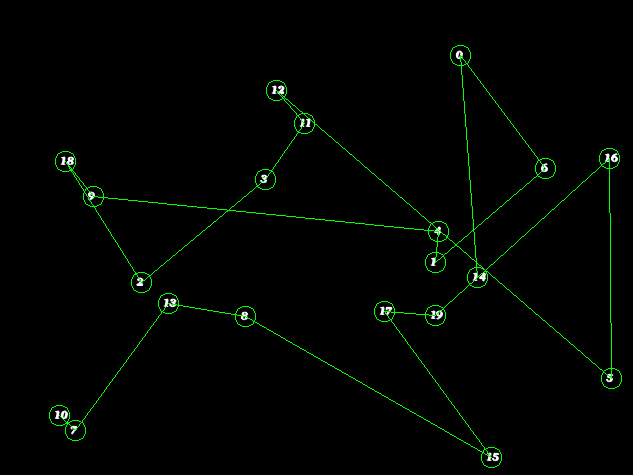
\includegraphics[width=\linewidth, height=8cm]{img/init.png}
        \caption{Initial problem with 20 nodes}
        \label{fig:init}
    \end{figure}
    \begin{figure}
        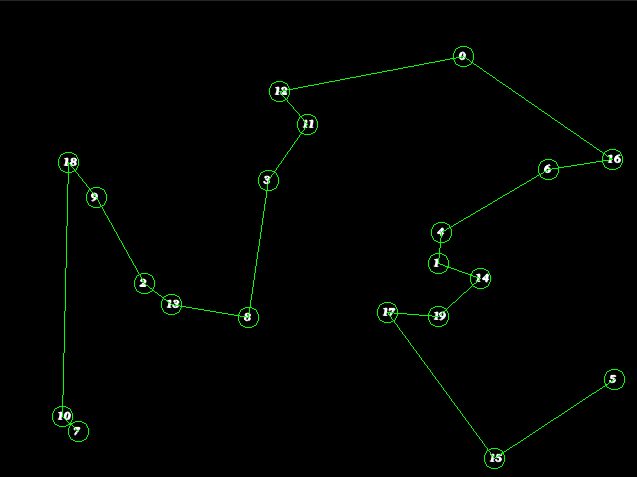
\includegraphics[width=\linewidth, height=8cm]{img/sol.png}
        \caption{Solution found after some iterations}
        \label{fig:sol}
    \end{figure}

    \section{A first approach}\label{sec:s2}
	The first approach that I though was to use the fact that we can divide each iteration in two phases, and each phase is parallelizable with a map. It was a pipeline with feedback composed by a map-reduce to calculate the affinity of each path by inverting the length with a reduce phase to compute the sum and to normalize each affinity in order to obtain proper probabilities and another map for the reproduction stage. Each worker had its own chunk of the population/affinities to compute, and the fastflow version was implemented with a parallelforreduce to compute the length of each path and to reduce on the sum, and another parallelfor to compute the new population.
    \begin{figure}
        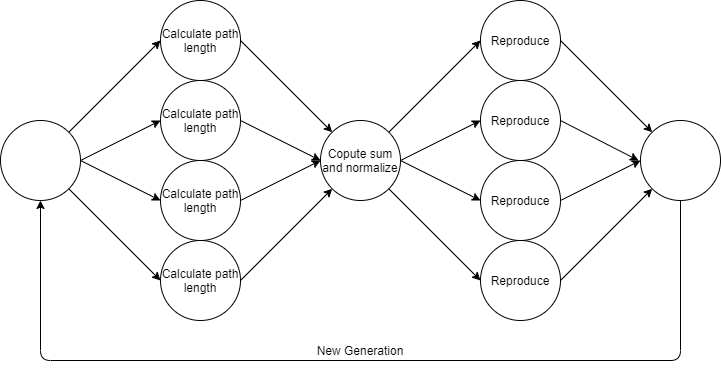
\includegraphics[width=\linewidth]{img/first.png}
        \caption{The first approach}
        \label{fig:first}
    \end{figure}
    This approach ideally reduces the completion time by a factor of nw, but it needs to have a barrier between the two phases and this leads to a lower speedup, because I need to have proper probabilities for the second stage to be executed. The good of this approach is that we have just one population with always the same size, independently by the number of workers and so taking in account crossovers with every possible pairs of the entire population. But the synchronization and the reduction are a bottleneck for this kind of skeleton. Due the fact that it is a pipeline of farm, I could apply a map fusion, using the sum as an accumulator state, and move from a stateful skeleton to a stateless one with a modification to the initial problem. When the population is big, the probabilities are all small and not very different because the path lengths don't differ too much, so the probabilities become less meaningful as the population increases (but anyway useful to keep the correctness of the algorithm). If I assume to have more than one independent populations where each one tries to solve the problem, I will not make the same computation as before because I won't be considering anymore the possibility of crossover among each pair of chromosomes of the enitre population, but I will get rid of the synchronization among workers, increasing performances and decreasing the completion time.

    \section{The second approach}\label{sec:s3}
	This approach is a simple farm over the task \textbf{evolve}, which is a composition of the two stages \textbf{calculate affinities} and \textbf{reproduce}. This composition is also known as\textbf{normal form}, and ensures the best performances with the lowest number of resources. In this way, we don't need to reduce on the sum.
Considering that, provided enough iterations i, the scheduler and the gatherer times are negligible (the emitter just have to pass the parameters to the workers, and the gatherer just have to find the best solution over the nw solutions returned by the nw workers), the completion time is

	\centerline{$i*T_{w}/nw$}

    So, by increasing the number of workers, I expect to see a linear speedup. My machine has 5 cores, so I also expect to have the \textbf{knee} at 5 workers. The heaviest data structure is the \textbf{population} one, which has dimension 0.08MB (4 byte(int) * 20 * 1000), while affinities has size 0.008MB (8byte(double) * 1000) and city as a very small size around 320byte (8byte(double) * 2 * 20 and 20*20 bit for the adjacent matrix). My cpu has 3 caches L1, L2 and L3 of size respectively 9MB, 1.5MB and 350KB, so data easily fits the L3 cache and I don't expect a superlinear speedup for cache fitting reasons.
    Anyway, I implemented the pick\_candidate function to cost O(n) in the worst case, where n is the population size, because it generates a random float and decreases it with the probabilities one after the other untill it becomes negative, and then the algorithm selects the candidate as the number of iterations needed. This could generate a superlinear speedup, because increasing the number of workers, we are not reducing only the number of chromosomes that each worker has to generate, but also the time needed to generate each of them.

    \begin{figure}
        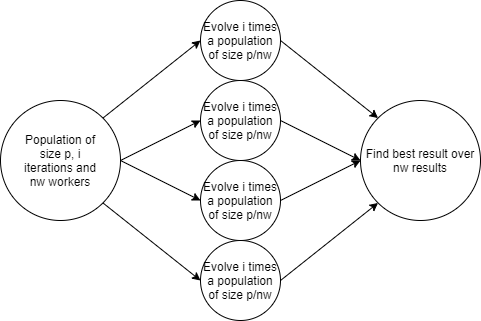
\includegraphics[width=\linewidth, height=8cm]{img/second.png}
        \caption{Second and final approach}
        \label{fig:second}
    \end{figure}


        \begin{table}[h!]
            \begin{center}
                \caption{Measured completion time, real completion time, gap between the two and gap percentage w.r.t. measured time for local execution with 20 nodes, 1000 chromosomes and 1000 iterations (time in microseconds). My machine has 5 cores.}
                \label{tab:table1}
                \begin{tabular}{c|c|c|c|c}
                    \textbf{nw} & \textbf{T(nw)} & \textbf{(T(1)/nw)} & \textbf{gap} & \textbf{T(nw)/gap}\\
                    \hline
                        1 & 8884752 & 8884752 & 0 & 0\%\\
                        2 & 4187312 & 4442376 & -255064 & -6\%\\
			3 & 2730646 & 2961584 & -230938 & -0.8\%\\
			4 & 2004171 & 2221188 & -217017 & -10\%\\
			5 & 1609943 & 1776950 & -167007 & -10\%\\
			6 & 1644261 & 1480792 & 163469 & 9.94\%\\
			7 & 1718324 & 1269250 & 449074 & 26.13\%\\
                \end{tabular}
            \end{center}
        \end{table}


    \begin{figure}
        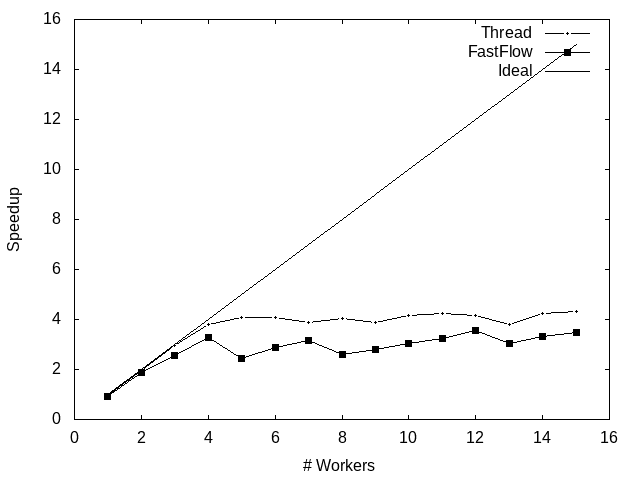
\includegraphics[width=\linewidth, height=8cm]{img/local_speedup.png}
        \caption{Local speed obtained with 20 nodes, 1000 chromosomes, 1000 iterations and 5 cores}
        \label{fig:locals}
    \end{figure}

    \begin{figure}
        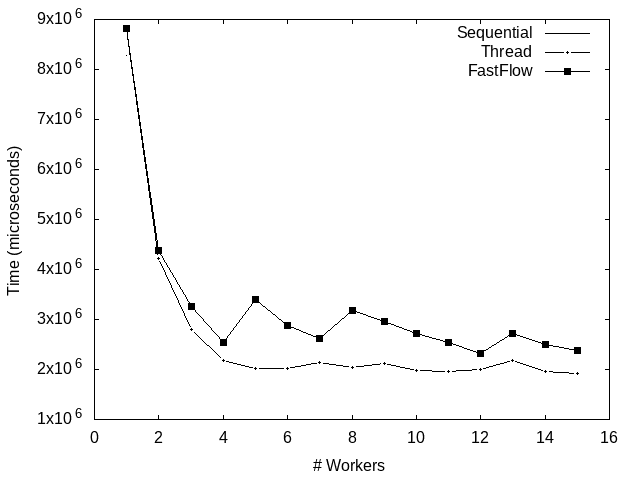
\includegraphics[width=\linewidth, height=8cm]{img/local_time.png}
        \caption{Local time obtained with 20 nodes, 1000 chromosomes and 1000 iterations and 5 cores}
        \label{fig:localt}
    \end{figure}

    \begin{figure}
        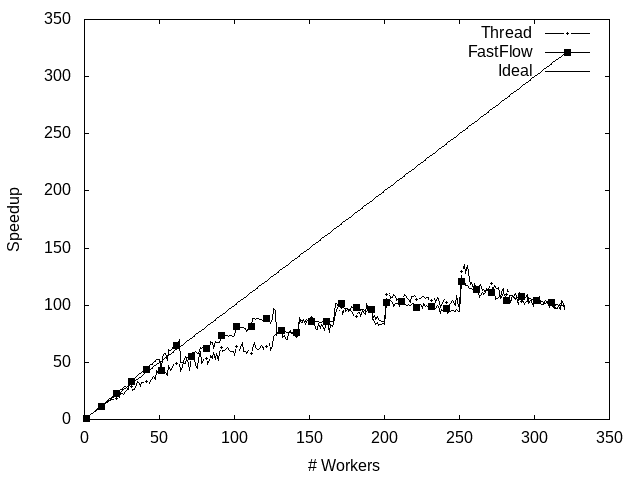
\includegraphics[width=\linewidth, height=8cm]{img/remote_speedup.png}
        \caption{Remote speedup obtained in phi19 machine, with 20 nodes, 1000 chromosomes, 1000 iterations and 256 cores}
        \label{fig:remotes}
    \end{figure}

    \section{Performance discussion}
	As we can see from the plots, in both the local and remote machines we have the knees in the expected points: at 5 in the local speedup because my machine has 5 cores and at 256 in the remote machine because it has 256 cores. The gap between the real speedup and the ideal one can be motivated by overheads, so the time needed to generate each thread (which becomes not negligible when nw gets higher) and the time to join them and to get the best results over the nw ones. The thread version is faster w.r.t. the FastFlow one because uses standard mechanisms of c++, which have less overheads w.r.t. the FastFlow library, even if the computation model is exactly the same.

    \section{Difficulties}
	At a certain point, I had a bottleneck in the remote machine that doesn't allow me to have a speedup higher than 3. I investigated this problem for days to find out that my bottleneck was caused by the \textbf{rand()} function, that I used for the crossover and mutation functions, and so it was called a lot of times every cycle. This, together with the pick candidate, made my development and my analysis a lot more difficult. To overcome this issue, I created the MyRandom class, which sets up just once for every worker the 3 differents uniform distribution that I used in the program, which are [0, n\_nodes)(int), [0, pop\_size)(int) and [0, 1](double).
	I didn't create the graphical visualization at runtime for the parallel versions because to do it I should have changed my stateless skeleton to a stateful one with a resource shared state composed by the shortest path length found and the relative shortest path, with an huge impact on the performances, that would have limited my speedup to the ratio $T_{w}/T_{state access}$.

    \section{Other improvements}
	I always compile my code with the -O3 flag in order to make other optimizations, like vectorization, which occours in various part of the code: when we push work in the farm of FastFlow, in the main loop of the Evolution node of FastFlow (basic block), in the affinities normalization, in the main loop of the thread (basic block), in the normalization of the sequential part, in the loop that starts the thread and in the loop that generates the population. Vectorization cannot happens in the main loop, because we need an \textbf{if} statement to check if the path just generated is the best found untill now. I tried to parallelize other part of the code, for example the random inizialization of the city and of the population, but I didn't get any improvements, so I removed it. The code can be optimized more, in the algorithmic way by rewriting the pick\_candidate function with a manipulation of the probabilities and using the binary search, or selecting the candidates with another approach, for example using an heap or by sorting them.

    \section{Conclusions}
	I experimented first to preserve the flow of the algorithm with the usage of synchronization between stages and shared vector (that could also raise false sharing issues), then I decided to generate more smaller flows of execution of the algorithm in order to get the best result at the end of the computations. If we want to see which is the best path found from the workers at runtime, we have to be careful at the state access pattern, where the state is made by the best length and the best path. In the thread version, we can overcome this issue with the usage of a mutex around the block which controls (and possibly sets) the best state w.r.t. the new one, but then the maximum speedup reached would have been the ratio between Tw/Ta, where Ta is the time needed to access the state.

\end{document}
